\section{Related Work}
\label{sec:relatedwork}

%\subsection{Private Inference}
CryptoNets~\cite{gilad2016cryptonets} was the first to demonstrate using homomorphic encryption to protect client data during inference. 
%CryptoNets uses polynomial activations to polynomials (quadratic function). 
SecureML~\cite{mohassel2017secureml} focuses on privacy-preserving training of several machine learning models, including neural networks using a two-server protocol. 
While \cite{mohassel2017secureml} supports inference as well, it incurs high overheads by relying on generic MPC protocols. MiniONN~\cite{liu2017oblivious} generates multiplication triplets for each multiplication in a linear layer and combines that with GC protocol for ReLU activation functions. 
Gazelle~\cite{juvekar2018gazelle} uses an optimized HE scheme for linear layers and GC for non-linear layers. DELPHI~\cite{mishra2020delphi} further optimizes this protocol by moving the heavy cryptographic operations to an offline preprocessing phase and using only secret sharing for linear layers online. 
In DELPHI, select ReLU layers are replaced with quadratic functions and the authors propose a neural architecture search method (NAS) to determine which ReLU layers to replace. 
CryptoNAS~\cite{ghodsi2020cryptonas} defines a ReLU budget for private inference task and aims to find the best networks for a budget using NAS. A recent work SAFENet \cite{lou2021safenet} selectively replaces the channel-wise ReLUs with multiple degree polynomials and uses layer-wise mixed precision. 

\begin{figure}[t] \centering
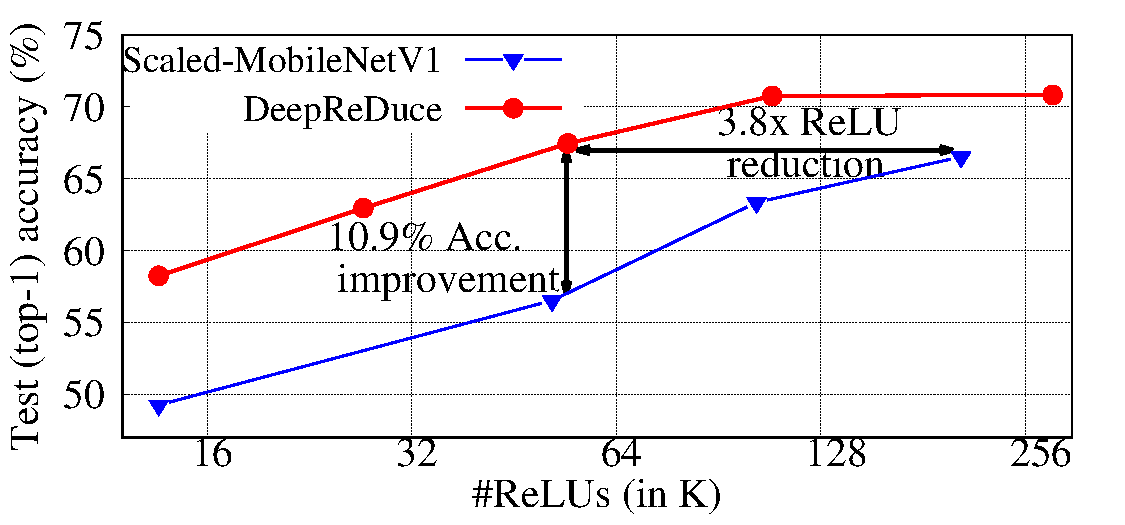
\includegraphics[scale=0.45]{Figures/ParetoFrontier_MV1}
%\vspace{-2.5em}
\caption{
Performance comparison of DeepReDuce models and (channel/fmap-resolution) scaled MobileNetV1 on CIFAR-100. DeepReDuce optimized models outperform the scaled MobileNetV1 by a huge margin at both iso-accuracy and iso-ReLU.}
%\vspace{-2em}
\label{fig:ParetoFrontierMV1}
\end{figure}


% \subsection{Effectiveness of ReLU} 
% Glorot et al.~\cite{glorot2011deep} first proposed the rectifier linear activation function, and the efficacy of ReLU for better convergence of deeper neural networks came into the limelight with the advent of AlexNet~\cite{krizhevsky2012imagenet}. Further, different versions of ReLU have been proposed mainly to overcome the issue of dead neurons and/or gradient vanishing/exploding \cite{maas2013rectifier,he2015delving,clevert2015fast,xu2015empirical,shang2016understanding,chen2020dynamic}.
% However, Zhao et al.~\cite{zhao2018reThinking} claimed that ReLU activations after each convolution layers creates redundancy and could lead to poor generalization. They showed a noticeable gain in accuracy when the network is trained with ReLUs in alternate convolution layers, which lines up with our empirical observation for dropping the ReLUs from alternate convolution layers in ReLU-stages.
 
 
% \subsection{Channel Pruning}
% Channel pruning is an effective way to reduce the FLOPs/parameter counts, and unlike the uniform channel scaling \cite{howard2017mobilenets,tan2019efficientnet}, ~\cite{wang2020apq,liu2019metapruning,he2018amc} proposed automatic pruning; however, their effectiveness for ReLU saving is yet to be examined since the distribution of FLOPs/parameters are substantially different from that of the ReLUs in the networks.

